\def\thecourse{18.466}
\def\thestudent{Zhilei Xu (929552018)}
\def\theprob{Midterm 2}
\documentclass[11pt]{article}
\usepackage{amsmath, graphicx, amsfonts}
\usepackage{fancyhdr}
\usepackage{lastpage}
\pagestyle{fancy}
\fancyhf{}
\fancyhf[HLEO]{\thestudent{}}
\fancyhf[HCEO]{\thecourse{} - Problem Set \theprob{}}
\fancyhf[HREO]{Page \thepage\ of \pageref{LastPage}}
\renewcommand\headrulewidth{0.4pt}
\newcommand{\argmax}{\mathrm{argmax}}
\newcommand\erf{\mathrm{erf}}
\newcommand\sgn{\mathrm{sgn}}
\newcommand{\widesim}[2][1.5]{
  \mathrel{\overset{#2}{\scalebox{#1}[1]{$\sim$}}}
}
\newcommand\eqnlabel[1]{\label{eqn:#1}}
\newcommand\eqnref[1]{(\ref{eqn:#1})}
\newcommand{\Beta}{\mathcal{B}}
\newcommand{\ProbS}{\iftrue}
\newcommand{\ProbE}{\fi}

\usepackage{titlesec, pgfplots, subcaption}
\titleformat{\section}[runin]{\Large\bfseries}{}{}{}
\titleformat{\subsection}[runin]{\normalfont\large\bfseries}{}{}{}
\begin{document}
\section*{1}
\subsection*{(a)}
$
\mu= E[X_i] = \frac{N+1}{2}
$,
so
$
\hat{N}_{MOM} =
2\bar{X}-1 = \frac{2}{3}(X_1+X_2+X_3)-1
$

\subsection*{(b)}
$
f(x | N) = \frac{I[x \leq N]}{N}, x=1,2,\dots
$,
so
$
f(X; N) = 
\frac{\prod_{i=1}^{3}I[X_i \leq N]}{N^3}
$,
hence
$
\hat{N}_{MLE} =
m = \max\{X_1, X_2, X_3\}
$

\subsection*{(c)}
$
Var[X_1] =
\left(\sum_{i=1}^{N} \frac{i^2}{N}\right) - \left(\frac{N+1}{2}\right)^2 =
\frac{(N+1)(2N+1)}{6} - \frac{(N+1)^2}{4} =
\frac{N^2-1}{12},
E[\hat{N}_{MOM}] =
E[2\bar{X}-1] = N
$, so
$
R(\hat{N}_{MOM},N) =
Var[\hat{N}_{MOM}] =
4Var[\bar{X}] =
\frac{4}{3} Var[X_1] = \frac{N^2-1}{9}
$.
\\
$
P_m(x) = P[m \leq x] = \prod_{i=1}^{3}P[X_i \leq x] =
\left(\frac{x}{N}\right)^3,
P[m = x] = \Delta P_m(x) =
\left(\frac{x}{N}\right)^3 -
\left(\frac{x-1}{N}\right)^3 =
\frac{3x^2-3x+1}{N^3}
$, \\
$
E[\hat{N}_{MLE}]=
\sum_{x=1}^{N} x\Delta P_m(x) =
[xP_m(x)] |_{0}^{N} - \sum_{x=1}^{N} P_m(x-1) \Delta x =
N P_m(N) - \sum_{x=1}^{N} P_m(x-1) =
$\\
$
N - \left(\sum_{x=1}^{N} (x-1)^3\right)/N^3 =
N - \left(\frac{N(N-1)}{2}\right)^2/N^3 =
\frac{(3N-1)(N+1)}{4N},
bias[\hat{N}_{MLE}] = \frac{-(N-1)^2}{4N}
$,\\
$
E[\hat{N}_{MLE}^2]=
\sum_{x=1}^{N} x^2\Delta P_m(x) =
\frac{\sum_{x=1}^{N} 3x^4 - 3x^3 + x^2}{N^3} =
\frac{(N+1)(36N^3+ 9N^2 - 19N + 4)}{60N^2},
Var[\hat{N}_{MLE}]=
\frac{(N^2-1)(9N^2-1)}{240N^2}
$ \\
$
R(\hat{N}_{MLE}, N) =
\frac{(N-1)^4}{16N^2} + 
\frac{(N^2-1)(9N^2-1)}{240N^2} =
%\frac{(N-1) ( 24N^3 - 36N^2 + 44N - 16 )}{240N^2}
%\frac{(N-1) ( 6N^3 - 9N^2 + 11N - 4 )}{60N^2}
\frac{(N-1) (2N-1) (3N^2-3N+4)}{60N^2}
$. Another direct way to compute: \\
Let
$
D = \hat{N}_{MLE}-N = m-N
$,
then
$
P[D=x] = P[m = x+N] =
\frac{3x^2 + (6N-3)x + (3N^2 - 3N + 1)}{N^3}
, 1-N \leq x \leq 0
$.\\
$
R(\hat{N}_{MLE}, N) =
E_N[D^2] =
\sum_{x=1-N}^{0} \frac{x^2[3x^2 + (6N-3)x + (3N^2 - 3N + 1)]}{N^3} =
\frac{(N-1)(2N-1)(3N^2 - 3N + 4)}{60N^2}
$. \\
Let
$
d(N) = {R(\hat{N}_{MOM}, N)} - {R(\hat{N}_{MLE}, N)} =
%\frac{60(N^2-1)N^2}{9(N-1)(2N-1)(3N^2-3N+4)} =
%\frac{N-1}{180N^2}\left[20N^2(N+1)-3(2N-1)(3N^2-3N+4)\right]
%\frac{N-1}{180N^2}\left[20N^3+20N^2-3(6N^3-3N^2 - 6N^2+3N + 8N-4)\right]
%\frac{N-1}{180N^2}\left[20N^3+20N^2-3(6N^3-9N^2 + 11N -4)\right]
%\frac{N-1}{180N^2}\left[20N^3+20N^2 -18N^3 +27N^2 -33N +12\right]
\frac{N-1}{180N^2}(2N^3+47N^2 -33N +12) =
\frac{N-1}{180N^2}f(N)
$,\\
$
f(1) = 28 >0,
\forall N \geq 1, f'(N) = 6N^2+94N-33 > 0
$, so
$
\forall N \geq 1, f(N)>0
$, \\
so we can see that
$
d(1) = 0
$
and
$
\forall N > 1, d(N) > 0
$. \\
So
$
\hat{N}_{MLE}
$
dominates
$
\hat{N}_{MOM}
$, 
and only when $N=1$, these two estimators have the same risk.

\iffalse
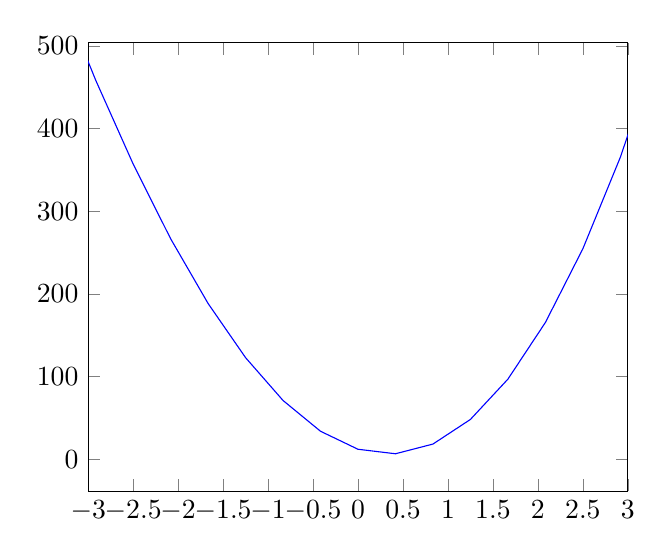
\begin{tikzpicture}
  \begin{axis}[
    xmin = -3,
    xmax = 3,
    xtick = {-3.0, -2.5, ..., 2.5, 3.0}
  ] 
  \addplot +[mark=none] {2*x^3+47*x^2-33*x+12}
  ;

  \end{axis}
\end{tikzpicture}
\fi

\subsection*{(d)}
The method of moment estimator can be improved by using the Rao-Blackwell theorem.\\
$
f(X; N) = 
\frac{\prod_{i=1}^{3}I[X_i \leq N]}{N^3} =
\frac{I[\max\{X_1, X_2, X_3\} \leq N]}{N^3}
$, so
$
m = \max\{X_1, X_2, X_3\}
$
is a sufficient statistic. \\
$
\hat{N}_{MOM} = 2\bar{X}-1 = \frac{2}{3}S-1
$, where
$ S=X_1+X_2+X_3$. \\
$
E[S | m] =
\sum_{i=1}^{m} P[X_1=i | m] \cdot E[S | m, X_1=i] =
$ \\
$
P[X_1=m | m] \cdot E[S | m, X_1=m] + \sum_{i=1}^{m-1} P[X_1=i | m] \cdot E[S | m, X_1=i] =
$ \\
$
\frac{m^2}{3m^2-3m+1}(m+E[X_2+X_3 | X_2 \leq m, X_3 \leq m]) + \sum_{i=1}^{m-1}\frac{2m-1}{3m^2-3m+1} \left(i+
E[X_2+X_3 | \max\{X_2, X_3\}=m]\right) =
$ \\
$
\frac{m^2(2m+1)}{3m^2-3m+1} + \frac{m(m-1)(2m-1)}{2(3m^2-3m+1)} +
\frac{(m-1)(2m-1)}{3m^2-3m+1}E[X_2+X_3 | \max\{X_2, X_3\}=m]
$

$
E[X_2+X_3 | \max\{X_2, X_3\}=m] =
$ \\
$
P[X_2 = m | \max\{X_2, X_3\}=m] \cdot (m+E[X_3 | X_3 \leq m]) +
\sum_{j=1}^{m-1}P[X_2 = j | \max\{X_2, X_3\}=m] \cdot (j+m) =
$ \\
$
\frac{m}{2m-1}(m+\frac{m+1}{2}) +
\frac{1}{2m-1} \cdot \frac{3m(m-1)}{2} =
\frac{3m^2-m}{2m-1}
$

So
$
E[S | m] =
\frac{m^2(2m+1)}{3m^2-3m+1} + \frac{m(m-1)(2m-1)}{2(3m^2-3m+1)} +
\frac{(m-1)(3m^2-m)}{3m^2-3m+1} =
\frac{3(2m^3-\frac{3m^2}{2}+\frac{m}{2})}{3m^2-3m+1}
$,\\
and the improved estimator
$
\hat{N}_{RB} = E[\frac{2}{3}S-1 | m] =
\frac{4m^3-3m^2+m}{3m^2-3m+1}-1 =
\frac{4m^3-6m^2+4m-1}{3m^2-3m+1} =
\frac{m^4-(m-1)^4}{m^3-(m-1)^3}
$ \\
$
E[\hat{N}_{RB}] =
\sum_{m=1}^{N} 
\frac{m^4-(m-1)^4}{3m^2-3m+1}
\cdot \frac{3m^2-3m+1}{N^3}
= N
$, so $\hat{N}_{RB}$ is unbiased. \\
$
E[\hat{N}_{RB}^2] =
\sum_{m=1}^{N} 
\frac{(m^4-(m-1)^4)^2}{(3m^2-3m+1)^2}
\cdot \frac{3m^2-3m+1}{N^3} =
\frac{1}{N^3}\sum_{m=1}^{N} 
\frac{(2m-1)^2(2m^2-2m+1)^2}{\frac{3}{4}(4m^2-4m+\frac{4}{3})} <
\frac{1}{N^3}\sum_{m=1}^{N} 
\frac{(2m-1)^2(2m^2-2m+1)^2}{\frac{3}{4}(4m^2-4m+1)} =
\frac{4}{3N^3}\sum_{m=1}^{N}(2m^2-2m+1)^2 =
\frac{4}{3N^3}\sum_{m=1}^{N}(4m^4-8m^3+8m^2-4m+1) =
\frac{4(4N^4+1)}{15N^2}
$, \\
$
R(\hat{N}_{RB}, N) = Var[\hat{N}_{RB}] <
\frac{4(4N^4+1)}{15N^2} - N^2 = \frac{N^4+4}{15N^2}
$. \\
For sufficiently large $N$ (such as $N \geq 3$),
$R(\hat{N}_{RB}, N)$ is close to $\frac{N^2}{15}$,
while $R(\hat{N}_{MOM}, N)$ is close to $\frac{N^2}{9}$,
so we can see that the method of moment estimator can be improved by using the Rao-Blackwell theorem.
For larger $N$, $R(\hat{N}_{MLE}, N)$ is close to $\frac{N^2}{10}$, so we can see that $\hat{N}_{RB}$ is even better than the maximum likelihood estimator for larger $N$.

\section*{2}
\subsection*{(a)}
Figures \ref{fig:linex}(\subref{fig:linex:0.2} - \subref{fig:linex:1}) are the plots for $l(\theta,a)$ as a function of $a-\theta$.
\begin{figure}[ht]
\centering
\foreach \c in {0.2, 0.5, 1} {
\subcaptionbox{c=\c \label{fig:linex:\c}}{
\begin{tikzpicture}
  \begin{axis}[
    xlabel={$a-\theta$},
    %ylabel={$l(\theta, a), c=\c$},
    xmin = -4.5,
    xmax = 3.5,
    xtick = {-4, ..., 3},
    width = 0.333\textwidth,
    height = 0.4\textwidth
  ] 
  \addplot +[mark=none] {e^(\c * x) - \c*x -1}
  %[yshift=8pt]
  %  node[pos=0.5] {$e^{\c(a-\theta)}-\c(a-\theta)-1$}
  ;
 
  \end{axis}
\end{tikzpicture}
}
}
\caption{plots for $l(\theta, a) = e^{c(a-\theta)}-c(a-\theta)-1$ as a function of $a-\theta$}
\label{fig:linex}
\end{figure}

\subsection*{(b)}
Lemma 1:
$
\forall A>0, t_m = -\log A
$
is the unique minimizer of
$
s(t) = Ae^t-t, t \in \{-\infty, +\infty\}
$. \\
Proof:
$s'(t) = Ae^t-1, s''(t) = Ae^t>0$.
$t_m = -\log A$ is the only root of $s'(t)=0$.
\\
Lemma 2:
For any random variable $\theta$ with distribution
$
\pi(\theta)
$,
the unique constant $a$ that minimizes
$
k(a) = \int_{\Theta} l(\theta, a) \pi(\theta)d\theta
$
is $a = -\frac{1}{c} E[e^{-c\theta}]$,
where
$
l(\theta, a) = e^{c(a-\theta)}-c(a-\theta)-1
$
and $E[\cdot]$ is taken w.r.t. $\pi(\theta)$.\\
Proof:
$
k(a) =
E[e^{c(a-\theta)}-c(a-\theta)-1] =
e^{ca}E[e^{-c\theta}]-ca - (cE[\theta]+1) =
Ae^{t}-t - B
$
\\
where
$
A=E[e^{-c\theta}],
B=cE[\theta]+1,
t=ca
$
and we require
$
c>0
$.
From Lemma 1 we know that the unique minimizer for $Ae^{t}-t$ is
$t_m=-\log A$, so the unique constant $a$ that minimizes $k(a)$ is
$a=-\frac{1}{c}\log E[e^{-c\theta}]$.

Now for any prior $\pi$ and estimator $V(X)$ of $\theta$,
the Bayes risk
$
r(V, \pi) =
\int_{\Theta} E_{\theta}[l(\theta, V(X))] \pi(\theta)d\theta
$ \\
$
= 
\int_{\Theta} \int_{\mathbf{X}} l(\theta, V(\mathbf{x})) f(\mathbf{x}|\theta) d\mathbf{x} \pi(\theta)d\theta
=
\int_{\mathbf{X}} \int_{\Theta} l(\theta, V(\mathbf{x})) f(\mathbf{x}|\theta)\pi(\theta)d\theta d\mathbf{x}
=
\int_{\mathbf{X}} \int_{\Theta} l(\theta, V(\mathbf{x})) \pi_{\mathbf{x}}(\theta)d\theta \tau(\mathbf{x})d\mathbf{x}
$ \\
where
$
\tau(\mathbf{x}) = \int_{\Theta} f(\mathbf{x} | \theta) \pi(\theta) d\theta \geq 0
$
does not depend on $\theta$,
$
\pi_{\mathbf{x}}(\theta) = \frac{f(\mathbf{x} | \theta)\pi(\theta)}{\tau(\mathbf{x})}
$
is the posterior distribution.\\
To minimize the double integral of $r(V, \pi)$, for any $\mathbf{x}$ in the outer integral, we need to minimize the corresponding inner integral.
In the inner integral with respect to $\theta$,
$\mathbf{x}$ is fixed and $\theta$ is a random variable with
the posterior distribution $\pi_{\mathbf{x}}(\theta)$.
To minimize this inner integral we need to choose $V(\mathbf{x})$, which would be constant for fixed $\mathbf{x}$, so by Lemma 2,
$V(\mathbf{x}) =
-\frac{1}{c}\log E_{\pi_{\mathbf{x}}}[e^{-c\theta}]
$ is the unique minimizer.

Thus the Bayes estimator of $\theta$ is
$
\delta^{\pi}(\mathbf{X}) =
-\frac{1}{c}\log E[e^{-c\theta} | \mathbf{X}]
$.

\subsection*{(c)}
The posterior distribution
$
\pi_X(\mu) \propto
\exp \left\{-\left[
\frac{(\mu-\eta)^2}{2\tau^2} +
\sum_{i=1}^{n} \frac{(\mu-X_i)^2}{2\sigma^2}
\right]\right\}
\propto
e^{-\frac{(\mu-m)^2}{2s^2}}
$, where \\
$
m= \frac{n\tau^2\bar{X} + \sigma^2 \eta}{n\tau^2 + \sigma^2}
,
s^2=\frac{\tau^2\sigma^2}{n\tau^2+\sigma^2}
$,
so $\pi_X$ must be a $N(m, s^2)$ distribution, its mgf
$
E_{\pi_X}[e^{t\mu}]= e^{mt+\frac{s^2t^2}{2}}
$.
\\
The Bayes estimator of $\mu$ under LINEX loss is
$
\hat{\mu} =
-\frac{1}{c} \log E[e^{-c\mu} | X] =
m-\frac{cs^2}{2} =
\frac{n\tau^2\bar{X} + \sigma^2 \eta - c\tau^2\sigma^2/2}{n\tau^2 + \sigma^2}
$

\section*{3}
Let
$
\delta(X) = X+1
$, then
$
E[\delta(X)] = E[X]+1 = 1/\theta
$, so it's unbiased.
$
Var[\delta(X)] = Var[X] = (1-\theta)/\theta^2
$

$
I(\theta) =
E_{\theta}\left[\left(\frac{\partial \log f}{\partial \theta}\right)^2\right] = 
E_{\theta}\left[\left(\frac{1}{\theta} - \frac{X}{1-\theta}\right)^2\right] =
\frac{1}{\theta^2} - \frac{2}{\theta(1-\theta)}E_{\theta}[X] +
\frac{1}{(1-\theta)^2}E_{\theta}[X^2] =
\frac{1}{\theta^2(1-\theta)}
$
\\
Let $g(\theta) = 1/\theta, g'(\theta)^2 = \theta^{-4}$.
Then for any $T$ -- unbiased estimator of $g(\theta)$,\\
$
Var_{\theta}[T] \geq g'(\theta)^2/I(\theta) = (1-\theta)/\theta^2 =
Var_{\theta}[\delta(X)]
$,
so $\delta(X)=X+1$ is UMVU estimator of $1/\theta$.

\section*{4}
\subsection*{(a)}
$
f(p_X, p_Y; X, Y) =
I[p_X \leq p_Y]
{n_X \choose X} p_X^{X} (1-p_X)^{n_X - X}
{n_Y \choose Y} p_Y^{Y} (1-p_Y)^{n_Y - Y},
0 \leq p_X \leq 1, 0 \leq p_Y \leq 1
$

Let
$
a(p) = 
 p^{X} (1-p)^{n_X - X},
b(p) =
 p^{Y} (1-p)^{n_Y - Y},
p \in [0, 1]
$.
$
g(p_X, p_Y) = a(p_X) b(p_Y),
p_X, p_Y \in [0, 1]
$.
\\
$
a'(p) = p^{X-1}(1-p)^{n_X-X-1}[X - n_X p]
$,
so $a'(p) > 0$ when $p \in [0, \frac{X}{n_X})$
(when $X=p=0$, $a'(p)=+\infty>0$),
and $a'(p) < 0$ when $p \in (\frac{X}{n_X}, 1]$,
hence $\tilde{p}_X=\frac{X}{n_X}$ uniquely maximizes $a(p)$.
\\
Similarly,
$b'(p) > 0$ when $p \in [0, \frac{Y}{n_Y})$,
$b'(p) < 0$ when $p \in (\frac{Y}{n_Y}, 1]$,
and $\tilde{p}_Y=\frac{Y}{n_Y}$ uniquely maximizes $b(p)$.

Clearly 
$(\tilde{p}_Y, \tilde{p}_Y)$ maximizes $g(p_X, p_Y)$,
and if
$p_X \leq p_Y$, then $(\tilde{p}_X, \tilde{p}_Y)$ also maximizes $f(p_X, p_Y; X, Y)$,
so we only need to consider the case when $\frac{X}{n_X} > \frac{Y}{n_Y}$,
and we argue that the maximizer of $f$ satisfies $p_X = p_Y$ in this case:
First, the maximizer of $f$ must satisfy $p_X \leq p_Y$.
Suppose $(p_X, p_Y)$ maximizes $f$ but does not satisfy $p_X=p_Y$, then $0 \leq p_X < p_Y \leq 1$.
If $p_Y < \frac{X}{n_X}$, then $p_X, p_Y \in [0, \frac{X}{n_X})$, so $a(p_Y) > a(p_X)$, and the pair $(p_X'=p_Y, p_Y)$ gives a greater likelihood than $(p_X, p_Y)$, contradicting the hypothesis that $(p_X, p_Y)$ maximizes $f$.
Otherwise $p_Y \geq \frac{X}{n_X} > \frac{Y}{n_Y}$, then we must have
$p_X = \frac{X}{n_X}$ (otherwise setting $p_X = \frac{X}{n_X}$ gives a greater likelihood), but again, in this case another pair $(p_X=\frac{X}{n_X}, p_Y'=p_X)$ gives a greater likelihood, contradicting the hypothesis.
So we have shown that in the case $\frac{X}{n_X} > \frac{Y}{n_Y}$, the maximizer of $f$ must satisfy $p_X=p_Y$, i.e. the problem of maximizing $f$ degenerates to maximizing
$h(p) = p^{X}(1-p)^{n_X-X} p^{Y} (1-p)^{n_Y-Y} = p^{X+Y} (1-p)^{n_X+n_Y-(X+Y)}$, with the obvious solution $\hat{p} = \frac{X+Y}{n_X+n_Y}$.

So the maximum likelihood estimator of $(p_X, p_Y)$ is
$
\left\{\begin{array}{cc}
\hat{p}_X = \frac{X}{n_X}, \hat{p}_Y = \frac{Y}{n_Y} & , \mathrm{when ~} \frac{X}{n_X} \leq \frac{Y}{n_Y}
\\
\hat{p}_X = \hat{p}_Y = \frac{X+Y}{n_X+n_Y} & , \mathrm{when ~} \frac{X}{n_X} > \frac{Y}{n_Y}
\end{array}\right.
$

\subsection*{(b)}
By Neyman-Pearson lemma, for $\alpha=0.05$, the MP level $\alpha$ test is the likelihood-ratio test
$$
\delta_c(X, Y) =
I\left[
\frac{0.6^{X}0.4^{n_X-X}0.75^{Y}0.25^{n_Y-Y}}
{0.5^{X}0.5^{n_X-X}0.5^{Y}0.5^{n_Y-Y}}
> c \right]
=
I\left[
%(3/2)^{X}(4/5)^{n_X}3^{Y}(1/2)^{n_Y}
(\frac{3}{2})^{X}(\frac{4}{5})^{n_X}3^{Y}(\frac{1}{2})^{n_Y}
> c \right]
=
I\left[
X\ln\frac{3}{2} + Y\ln3 > q_c
\right]
$$
where $q_c = \ln (\frac{5}{4})^{n_X} 2^{n_Y} c$, and $q_c$ is determined by
$
P_0 \left[
X\ln\frac{3}{2} + Y\ln3
> q_c
\right] = \alpha = 0.05
$.
Under null hypothesis, when $n_X$ and $n_Y$ are large, by Central Limit Theorem, $X$ and $Y$ approximately follow $N(\frac{n_X}{2}, \frac{n_X}{4})$ and $N(\frac{n_Y}{2}, \frac{n_Y}{4})$ respectively, so
$
X\ln\frac{3}{2} + Y\ln3
$
approximately follow
$
N(\frac{n_X}{2} \ln \frac{3}{2}+\frac{n_Y}{2}\ln3,
\frac{n_X}{4}(\ln\frac{3}{2})^2 + \frac{n_Y}{4}(\ln 3)^2)
$.
$$
0.05 = P_0 \left[
X\ln\frac{3}{2} + Y\ln3
> q
\right] \approx
1-
\phi\left(\frac{q-\frac{n_X}{2} \ln \frac{3}{2}-\frac{n_Y}{2}\ln3}
{\sqrt{\frac{n_X}{4}(\ln\frac{3}{2})^2 + \frac{n_Y}{4}(\ln 3)^2}}
\right)
\implies
q \approx 
\frac{n_X}{2} \ln \frac{3}{2}+\frac{n_Y}{2}\ln3+
\phi^{-1}(0.95)
\sqrt{\cdots}
%{\sqrt{\frac{n_X}{4}(\ln\frac{3}{2})^2 + \frac{n_Y}{4}(\ln 3)^2}}
$$
So the MP test is
$
\delta(X, Y) =
I\left[
X\ln\frac{3}{2} + Y\ln3 > q
\right]
$
where
$
q \approx 
\frac{n_X}{2} \ln \frac{3}{2}+\frac{n_Y}{2}\ln3+
1.645
{\sqrt{\frac{n_X}{4}(\ln\frac{3}{2})^2 + \frac{n_Y}{4}(\ln 3)^2}}
$. \\
For $X=15, n_X=30, Y=21, n_Y=30$,
%R code: q <- function(nx, ny) {nx * log(3/2) / 2 + ny*log(3)/2 + qnorm(1-0.05)*sqrt(nx*(log(3/2)**2)/4+ny*((log(3))**2)/4)}
% test <- function(x, y) {x*log(3/2) + y*log(3)}
% test(15, 21); q(30, 30)
$q \approx 27.83628, X\ln\frac{3}{2}+Y\ln3 \approx 29.15283 > q$, so reject $H_0$.

\subsection*{(c)}
There does \emph{not} exist a UMP test of
$H_0: p_X=p_Y=0.5$
vs.
$H_1: p_X<p_Y, p_X \geq 0.5$.

Suppose for some $\alpha \in (0, 1)$ there exists such a UMP level $\alpha$ test
$\delta$ for testing $H_0: p_X=p_Y=0.5$ vs. $H_1: p_X<p_Y, p_X \geq 0.5$, then it must also be MP test for testing
$
H_0 
$
vs.
$
H_1': p_X=0.6, p_Y=0.75
$
and for testing
$H_0$ vs.
$
H_1'': p_X=0.6, p_Y=0.8
$.

From part (b) we know that the MP level $\alpha$ likelihood ratio tests for the latter two test problems are \\
$
\phi(X, Y) = I[X\ln\frac{3}{2}+Y\ln3 > c]
$
and
$
\psi(X, Y) = I[X\ln\frac{3}{2}+Y\ln4 > d]
$
where $c$ and $d$ are constants determined by
$
P_0[X\ln\frac{3}{2}+Y\ln3 > c]
=
P_0[X\ln\frac{3}{2}+Y\ln4 > d]
=\alpha
$.

By Neyman-Pearson lemma, $\delta$ must be almost same as both $\phi$ and $\psi$, so $\phi$ and $\psi$ are almost same, too. But\\
$
P_0[\phi(X, Y) \neq \psi(X, Y)]
\geq
P_0[\phi(X, Y)=1 \wedge \psi(X, Y) = 0]
\geq
P_0[ X\ln\frac{3}{2}+Y\ln3 > c \wedge X\ln\frac{3}{2}+Y\ln4 < d]
>0
$
\\
contradicts the fact that $\phi$ and $\psi$ are almost same. The contradiction shows that our hypothesis is wrong, so there is no UMP test of $H_0: p_X=p_Y=0.5$ vs. $H_1: p_X<p_Y, p_X \geq 0.5$.

\section*{5}
This problem is so amazing! Only after solving it did I fully understand these sentences: Such randomized tests are not used in practice. They are only used to show that with randomization, likelihood ratio tests are unbeatable no matter what the size $\alpha$ is. [Bickel \& Docksum, p. 224]
\subsection*{(a)}
$
f(\theta; \mathbf{X}) =
\prod_{i=1}^{n} I[\theta \leq X_i \leq \theta+1] =
I[\min(X_1, \dots, X_n) \geq \theta \wedge \max(X_1, \dots, X_n) \leq \theta+1]
$
\\
Consider the test $H_0': \theta=\theta_0$ vs. $H_1': \theta=\theta_1$.
For any fixed $\theta_1 \in (\theta_0, \theta_0+1-\sqrt[n]{\alpha})$, the likelihood ratio \\
$
LR_{\theta_1/\theta_0} =
\frac{
I[\min(X_1, \dots, X_n) \geq \theta_1 \wedge \max(X_1, \dots, X_n) \leq \theta_1+1]
}
{
I[\min(X_1, \dots, X_n) \geq \theta_0 \wedge \max(X_1, \dots, X_n) \leq \theta_0+1]
} =
\left\{\begin{array}{cl}
+\infty & , \max(X_1, \dots, X_n) > \theta_0+1
\\
1 & , \min(X_1, \dots, X_n) \geq \theta_1 \wedge \max(X_1, \dots, X_n) \leq \theta_0+1
\\
0 & , \min(X_1, \dots, X_n) < \theta_1
\end{array}\right.
$

%If $\theta_1 > \theta_0+1$, it is further reduced to
%$
%LR_{\theta_1/\theta_0} =
%\left\{\begin{array}{cl}
%+\infty & , \max(X_1, \dots, X_n) > \theta_0+1
%\\
%0 & , Otherwise
%\end{array}\right.
%$
The likelihood ratio test
$
\varphi_1(\mathbf{X}) =
\left\{\begin{array}{cl}
1 & , \max(X_1, \dots, X_n) > \theta_0+1
\\
\frac{\alpha}{(\theta_0+1-\theta_1)^n} & , \min(X_1, \dots, X_n) \geq \theta_1 \wedge \max(X_1, \dots, X_n) \leq \theta_0+1
\\
0 & , \min(X_1, \dots, X_n) < \theta_1
\end{array}\right.
$
\\
is the MP level $\alpha$ test of $H_0'$ vs. $H_1'$.
Note that $\theta_1 \in (\theta_0, \theta_0+1-\sqrt[n]{\alpha})$ so
$0 < \frac{\alpha}{(\theta_0+1-\theta_1)^n} <1$,
hence $\varphi_1$ is indeed a randomized likelihood ratio test with critical value $1$.
It's also easy to verify that its size is $\alpha$.

Now let $C(\alpha)=1-\sqrt[n]{\alpha}$, the test
$
\delta(\mathbf{X}) =
I\left[
\min(X_1, \dots, X_n)>\theta_0+C(\alpha)
\vee
\max(X_1, \dots, X_n)>\theta_0+1
\right]
$
is UMP level $\alpha$ test for $H_0': \theta=\theta_0$ vs. $H_1': \theta=\theta_1$ where $\theta_1 \in (\theta_0, +\infty)$ is fixed.
First we know its size is
$
P_{\theta_0} \left[
\min(X_1, \dots, X_n)>\theta_0+C(\alpha)
\vee
\max(X_1, \dots, X_n)>\theta_0+1
\right] =
P_{\theta_0} \left[
\min(X_1, \dots, X_n)>\theta_0+1-\sqrt[n]{\alpha}
\right] =
\left[(\theta_0+1)-(\theta_0+1-\sqrt[n]{\alpha})\right]^n = \alpha
$.
Next we calculate its power by cases:\\
1. If $\theta_1 \geq \theta_0 + 1-\sqrt[n]{\alpha}$, then
$
\beta(\delta) =
P_{\theta_1} \left[
\min(X_1, \dots, X_n)>\theta_0+C(\alpha)
\vee
\max(X_1, \dots, X_n)>\theta_0+1
\right] = 1
$,
so $\delta$ is obviously UMP test for $H_0'$ vs. $H_1'$.
\\
2. Otherwise $\theta_1 \in (\theta_0, 1-\sqrt[n]{\alpha})$, then
$
\beta(\delta) =
P_{\theta_1} \left[
\min(X_1, \dots, X_n)>\theta_0+C(\alpha)
\vee
\max(X_1, \dots, X_n)>\theta_0+1
\right] =
P_{\theta_1} \left[
\min(X_1, \dots, X_n)>\theta_0+1-\sqrt[n]{\alpha}
\wedge
\max(X_1, \dots, X_n) \leq \theta_0+1
\right] +
P_{\theta_1} \left[
\max(X_1, \dots, X_n) > \theta_0+1
\right] =
$\\
$
1-(\theta_0+1-\theta_1)^{n} + \alpha
$. On the other hand, it's easy to calculate that the size $\alpha$ likelihood ratio test
$
\varphi_1
$
(which is UMP) has exactly the same power. Thus $\delta$ is again UMP for $H_0'$ vs. $H_1'$.

So now we have proved that $\delta$ is UMP level $\alpha$ test for $H_0': \theta=\theta_0$ vs. $H_1': \theta=\theta_1$ where $\theta_1 \in (\theta_0, +\infty)$ is fixed. Next we prove $\delta$ is also UMP for $H_0: \theta \leq \theta_0$ vs. $H_1: \theta > \theta_0$. This is easy:
First it is easy to verify that the size of $\delta$,
$\alpha(\delta) = \sup_{\theta \in (-\infty, \theta_0]} \{
P_{\theta} \left[
\min(X_1, \dots, X_n)>\theta_0+C(\alpha)
\vee
\max(X_1, \dots, X_n)>\theta_0+1
\right] \} =
P_{\theta_0} \left[
\min(X_1, \dots, X_n)>\theta_0+1-\sqrt[n]{\alpha}
\vee
\max(X_1, \dots, X_n)>\theta_0+1
\right] = \alpha
$,
so $\delta$ is indeed a level $\alpha$ test for $H_0$ vs. $H_1$.
Next suppose $\delta$ is not UMP for $H_0$ vs. $H_1$, then there exists another test $\varphi$ such that its size $\alpha(\varphi) \leq \alpha$ and for some $\theta_1 > \theta_0$, when $\theta=\theta_1$, $\beta(\varphi) > \beta(\delta)$. But this $\varphi$ must also be a level $\alpha$ test for $H_0': \theta=\theta_0$ vs. $H_1': \theta=\theta_1$ whose power is greater than $\delta$, contraditing the proven fact that $\delta$ is UMP level $\alpha$ test for $H_0'$ vs. $H_1'$.

To sum up: the test $\delta$ which rejects when
$
\min(X_1, \dots, X_n) > \theta_0 + C(\alpha)
$
or
$
\max(X_1, \dots, X_n) > \theta_0 + 1
$
where
$
C(\alpha) = 1-\sqrt[n]{\alpha}
$
is a UMP level $\alpha$ test for testing $H_0: \theta \leq \theta_0$ vs. $H_1: \theta > \theta_0$.

\subsection*{(b)}
Suppose this family has monotone likelihood ratio in some statistic $T(\mathbf{X})$, i.e. \\
$
\forall \theta_1, \theta_0 ~ s.t. ~ \theta_1>\theta_0,
LR(\mathbf{X}, \theta_0, \theta_1) =
\frac{f(\theta_1; \mathbf{X})}{f(\theta_0; \mathbf{X})}
$
is increasing with $T(\mathbf{X})$.
Then the level $\alpha$ UMP likelihood ratio test for testing
$
H_0: \theta = \theta_0
$
agains
$
H_0: \theta > \theta_0
$
reduces to
$
\varphi_{c} = \left\{\begin{array}{cl}
1 & ,T(\mathbf{X}) > c(\alpha) \\
r_{\alpha} & ,T(\mathbf{X}) = c(\alpha) \\
0 & ,T(\mathbf{X}) < c(\alpha)
\end{array}\right.
$
where
$
c(\alpha)
$
is the \emph{critical value} which is related to both $\alpha$ and $\theta_0$,
$
0<r_{\alpha}<1
$ corresponds to the randomized decision.
For any fixed $\theta_0$, varying $\alpha$ from $0$ to $1$ continuously induces a set of UMP likelihood tests with critical values $c$ varying from $-\infty$ to $+\infty$ continuously. If we only care about the deterministic decisions, then this set
$S(\theta_0)$ is the same for different values of $\theta_0$, so we just call it $S$.

For any fixed $\theta_0$ and $\alpha \in [0, 1]$, let $\delta_{\theta_0, \alpha}$ denote the UMP level $\alpha$ test derived in part (a) for testing $H_0: \theta=\theta_0$ vs. $H_1: \theta>\theta_0$,
then by Neyman-Pearson lemma, there exists a likelihood ratio test $\varphi_{c} \in S$, such that
%$
%\forall \theta \geq \theta_0,
%P_{\theta}[\delta_{\theta_0, \alpha}(\mathbf{X}) \neq \varphi_{c}(\mathbf{X}) \wedge T(\mathbf{X}) \neq c] = 0
%$, and we call the two tests
$\delta_{\theta_0, \alpha}$ and $\varphi_{c}$ are ``\emph{almost same}''.
Let
$
D(\theta_0) = \{ \delta_{\theta_0, \alpha} | \alpha \in [0, 1] \}
$
denote the set of UMP tests derived in part (a) with level $\alpha$ varying from $0$ to $1$ continously, for a fixed $\theta_0$, then $D(\theta_0)$ must be almost same as $S$, so for different $\theta_0 \neq \theta_0'$, $D(\theta_0)$ and $D(\theta_0')$ must be almost same, too.

Now for the sets $D(0)$ and $D(2)$ and $\alpha = 0.1$,
$\delta_{2, \alpha} \in D(2)$ and we argue that there is no $\delta_{0, \alpha'} \in D(0)$ such that $\delta_{2, \alpha}$ and $\delta_{0, \alpha'}$ are almost same: For any $\alpha \in (0, 1), \alpha' \in [0, 1]$,\\
$
\delta_{2, \alpha}(\mathbf{X}) = I[\min(X_1, \dots, X_n) > 3-\sqrt[n]{\alpha} \vee \max(X_1, \dots, X_n) > 3]
$
\\
$
\delta_{0, \alpha'}(\mathbf{X}) = I[\min(X_1, \dots, X_n) > 1-\sqrt[n]{\alpha'} \vee \max(X_1, \dots, X_n) > 1]
$
\\
$
P_{\theta=2}[\delta_{2, \alpha}(\mathbf{X}) \neq \delta_{0, \alpha'}(\mathbf{X})]
\geq
P_{\theta=2}[\delta_{2, \alpha}(\mathbf{X})=0 \wedge \delta_{0, \alpha'}(\mathbf{X})=1]
=
$
\\
$
P_{\theta=2}[
\min(X_1, \dots, X_n) \leq 3-\sqrt[n]{\alpha} \wedge \max(X_1, \dots, X_n) \leq 3
] > 0
$
\\
So any $\delta_{0, \alpha'} \in D(0)$ cannot be almost same as $\delta_{2, \alpha} \in D(2)$, hence the two sets $D(0)$ and $D(2)$ cannot be almost same, contradicting the proven fact that for any $\theta \neq \theta'$, $D(\theta)$ and $D(\theta')$ must be almost same.

The contradiction shows that our hypothesis is wrong, so the family $\mathbf{X} \widesim{i.i.d.} Uniform(\theta, \theta+1)$, \\
$-\infty < \theta < \infty$ does not have monotone likelihood ratio in any statistic $T(\mathbf{X})$.

\end{document}
